\chapter{Analysis for Concurrent Programs}

We will be using the technique mentioned in the paper Dataflow Analysis for Datarace-Free Programs\cite{Arnab2006}. This technique when given a sequential data-flow analysis produces an efficient and fairly precise analysis for concurrent programs. The criteria to be met for applying this analysis is that data-flow fact should  be dependent on the contents of the associated lvalues (expression referring to memory location at runtime). Sequential analysis like null-pointer analysis, interval analysis and constant propagation. In terms of precision of the data-flow facts, useful information will be derived at program points where the lvalue is read.\cite{Arnab2006} \\

The main challenge in converting the analysis from sequential to concurrent programs is that propagating data-flow values such that all the possible concurrent executions of the thread are taken care of. In this technique, the synchronization structure of the program is made use of to propagate data-flow values. The main insight used is that the data-flow values are only propagated between threads at the lock and unlock points in threads for access to critical sections. Also this approach will not work for programs containing data race. \\

\section{Memory Model and Data Races}

We will model the notion of concurrency in programs using threads at the moment. The shared variables in the thread will be accessed inside a pair of lock and unlock statements. Note that, this only covers the case in which only one thread can execute in the critical section. We have not modeled the case of general semaphores in which multiple threads can execute inside the critical sections. \\

A memory model specifies the interactions of threads with memory and its shared use. Thus , memory model specify the constraints on data access and conditions on how data written by one thread is accessible to other threads. Happens before is the memory model described in the paper and thesis on Concurrent Program analysis. \\ 


The happens before memory model is based on the happens-before relation which relates the happenings of two events such that if one happens before the other, it should be reflected in the results. That is if statement A occurs before statement B then the memory written by statement A is visible to statement B. \\
There are three components of the happens before memory model.
\begin{enumerate}
	\item Program Order: It is generally used to refer to the order of statement in a thread as they appear in the program. However the formal definition of program order is the intra-thread order during the execution of the program.
	\item Synchronizes-with Relation: This relation is defined over synchronization relations which are lock, unlock (for acquiring/releasing locks), spawn, join (to synchronize creation/endind of multiple threads), start, end(first/last statement of a thread). The synchronizes-with relation is defined from
	\begin{itemize}
		\item Lock statement to all previous unlock statements
		\item A begin statement to the spawn statement of the thread
		\item Join statement to the end statements of all the threads synchronized
	\end{itemize} 
	\item Happens-Before Order: Statement  a happens before statement b if one of the following hold
	\begin{itemize}
		\item a appears before b in the program order
		\item b synchronizes-with a
		\item b can be reached transitively using happens-before relation from a.
	\end{itemize}   
\end{enumerate}
 
\begin{figure}
	\centering
	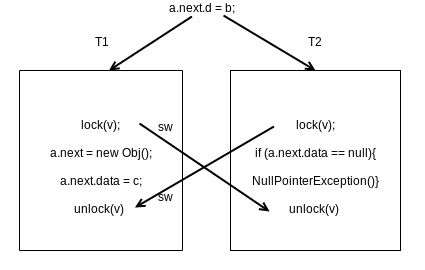
\includegraphics[width=0.6\textwidth]{Figures/sync_threads.png}
	\caption{Happens Before memory model with thread synchronization}
	\label{fig:happensbefore1}
\end{figure}


\begin{figure}[b]
	\centering
	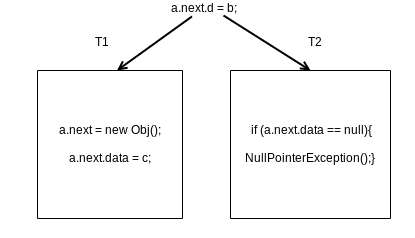
\includegraphics[width=0.5\textwidth]{Figures/sync_no_lock.png}
	\caption{Happens Before memory model without thread synchronization}
	\label{fig:happensbefore2}
\end{figure} 
 
Consider the example presented in Figure 4.1. We have an example of 2 threads executing the critical section. Assume that \emph{a.next} was initially pointing to an object $o_i$ on the heap which contains non-null data. We need to check if the exception in $T_2$ can be thrown. Applying the happens-before relation, we can find out this will never be the case. The synchronization of locks and unlocks always prevents the possibility of \emph{a.next} pointing to a dynamically created object with \emph{null} when the \emph{if} condition in $T_2$ is checked, irrespective of any possible thread scheduling. The exception would only have been raised if the statement 2 of T \\

Now consider the case given in Figure 4.2. It has the same statements but does not contain proper locking and hence no synchronization edges. So in this case all the actions in T1 need not happen before the evaluation of the condition. The exception can now thrown be in case the execution order is {($T_1$,$s1$),($T_2$,$s2$)}. This necessitates data race free program as input to the analysis.\\


Data Race : A data race occurs when two or more threads can access shared data at the same time and try to change it at the same time. Also the order of access among the threads will not be known, so both the threads are racing to access or modify the shared data. Formally, a data race is said when

\begin{enumerate}
	\item Two or more threads access the same memory location concurrently
	\item At least one of the accesses is a write
	\item he threads are not using any exclusive locks to control their accesses to that memory.
\end{enumerate}

Data race can be defined in terms of happens before relation. Two statements are said to be conflicting/racy if neither a happens before b or b happens before a. We will only deal with programs which are data race free. 

\section{Concurrent analysis technique}

Arnab De has explained his approach to concurrent data flow analysis\cite{Arnab2006} by giving example of access path based null-pointer analysis. He argues that the data-flow value is true only before the statement where the corresponding access path/lvalue is relevant. \\

The first step in the analysis is to add edges between nodes of control flow graph representing different threads. These edges map to the synchronize-with edges in the happens before memory model. Hence, the name sync-CFG is given to this control flow graph. The edges are added from the spawn statement to the first statement of each thread, from the unlock statement to lock statement if they access the same lock variable and  belong to different threads. In the next step sequential data flow analysis is performed on the syn-CFG. The synchronization edges have identity flow functions. The example of the access-path based null pointer analysis inspired from\cite{Arnab2006} is in Figure 3.1 \\

\begin{figure}
	\centering
	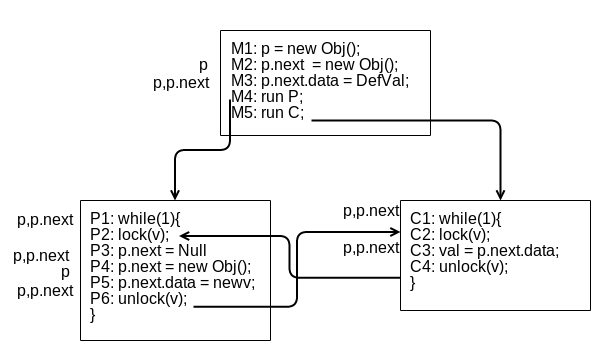
\includegraphics[width=0.6\textwidth]{Figures/concurrent_analysis.png}
	\caption{Heap Access path based null pointer analysis}
	\label{fig:nullpointeranalysis}
\end{figure}


In Figure 3.1 the synchronization edges are added to generate the sync-CFG.It also shows access paths to memory locations which are discovered to be not null by the analysis. The values are marked in italics for each corresponding statement. As p.data is non-null at point $M_5$ in the main thread before spawning the cons thread, this value gets propagated to the first instruction $C_1$ of the cons thread though one of the added edges, and from there to the lock instruction at $C_2$. Similarly, although \emph{p.next} is set back to non-null at $P_4$ before the unlock, despite being set to
null at $P_3$ in the prod thread. This fact also gets propagated to the lock statement of the cons thread through the edge from $P_6$ to $C_2$. As p.next is not null in both the paths joining at $C_2$, we can conclude \emph{p.next} to be non-null before the lock statement in all executions by the merge operation. \\

An important point to note about this technique is that, it may compute incorrect values at program points not containing access paths. For all data-race free programs, relevant statements will occur in the lock-unlock regions. Those statements containing access path or reference expression are considered relevant. In the given example $C_1$ is not a relevant statement and the data flow value \emph{p.next} is incorrect considering the program execution order [$P_3$ $C_1$]. %An example that can be designed to provide as input for concurrent heap liveness analysis is shown in Figure 4.4. 

\section{Concurrent Heap Liveness Analysis}

Consider the Example shown in Figure 4.4, showing the first iteration. Heap  liveness analysis is a backward flow problem. Figure 4.5, 4.6,4.7 shows the data flow values after iterations 2,3 and 4 respectively. At the beginning of $s_1$ in Thread 1, the live access path are \emph{x.f1.r}, \emph{x.f1.f2.r}. This is approximated by the access graph shown in Figure 4.7. Access graph representation is essential to represent finitely, the access paths(especially in the case of presence of loops). The synchronization edges introduce a structure similar to loops in the sync-cfg. Thus paths like \emph{x.f1.f2.f1.r} and \emph{x.f1.f2.f1.f2.r} are marked out to be live. We will obtain extra spurious live access paths by adding sync-edges, however the access graph will contain all the valid live paths at a point inside the lock-unlock statements. Also , note that at the start of the main statement, \emph{x.f1.r},\emph{x.f2.r}. \emph{x.f1.f2.r} and \emph{x.f2.f1.r} paths are live.\\

Figure 4.8 shows the heap liveness analysis performed without adding the synchronization edges in the cfg. This will just mark out the access path \emph{x.f1.r} live at the starting of $s_1$ in Thread 1. The absence of synchronization edges misses out the liveness of the access path \emph{x.f1.f2.r} at the starting of $s_1$ in Thread 1. The access graph at the start of the statement main is same even without the effect of synchronization edges for this example. Even without synchronization edges,the access paths \emph{x.f1.r},\emph{x.f2.r}. \emph{x.f1.f2.r} and \emph{x.f2.f1.r} are live. \\

Figure 4.9 illustrates the an input cfg that needs to be given as input to the concurrent heap liveness analysis. We also  need to handle procedure calls inside the lock-unlock statements, using the value contexts method. \\

In the next chapter we will be discussing the problems with this analysis method. The fact that analysis without adding synchronization edges gives better liveness data flow value, highlights that there are some problems with this analysis. We will discuss them in greater detail in the next chapter. 

\begin{figure}
	\centering
	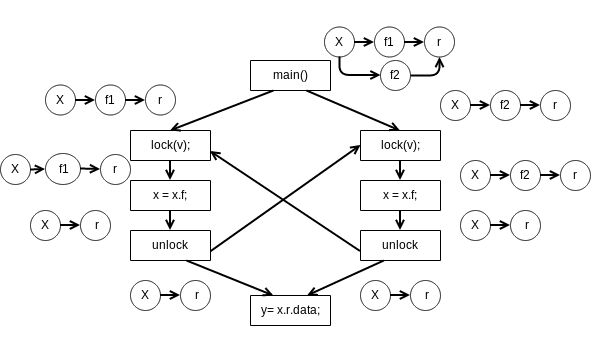
\includegraphics[width=0.8\textwidth]{Figures/conc_analysis_itr1.png}
	\caption{Concurrent Heap liveness analysis iteration 1}
	\label{fig:nullpointeranalysis}
\end{figure}

\begin{figure}
	\centering
	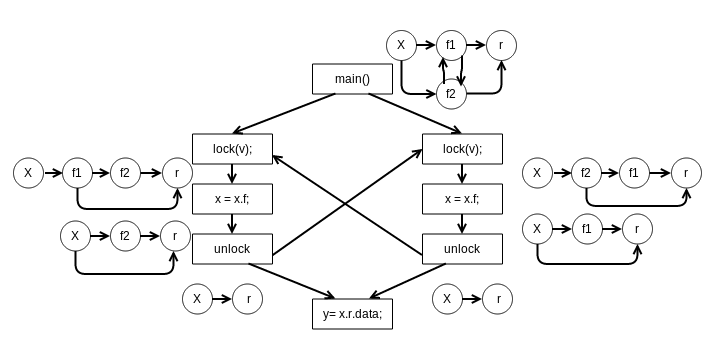
\includegraphics[width=0.8\textwidth]{Figures/conc_analysis_itr2.png}
	\caption{Concurrent Heap liveness analysis iteration 2}
	\label{fig:nullpointeranalysis}
\end{figure}

\begin{figure}
	\centering
	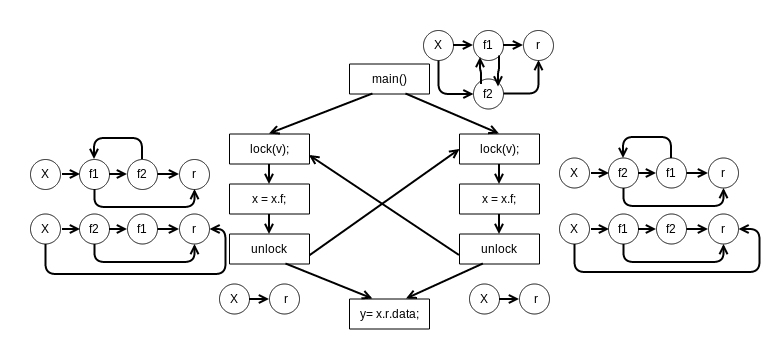
\includegraphics[width=0.8\textwidth]{Figures/conc_analysis_itr3.png}
	\caption{Concurrent Heap liveness analysis iteration 3}
	\label{fig:nullpointeranalysis}
\end{figure}

\begin{figure}
	\centering
	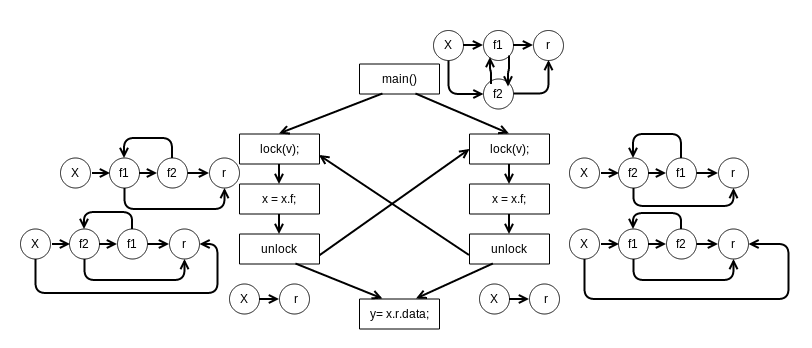
\includegraphics[width=0.8\textwidth]{Figures/conc_analysis_itr4.png}
	\caption{Concurrent Heap liveness analysis iteration 4}
	\label{fig:nullpointeranalysis}
\end{figure}

\begin{figure}
	\centering
	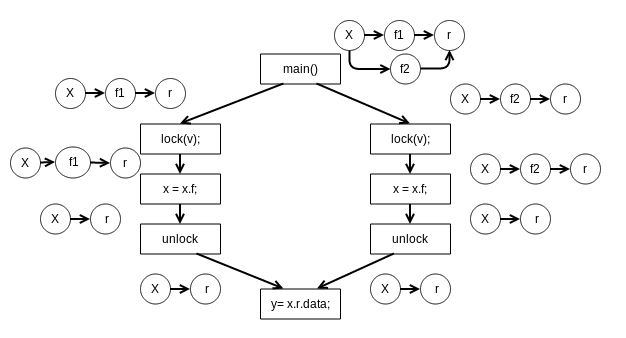
\includegraphics[width=0.8\textwidth]{Figures/conc_analysis_incorrect.png}
	\caption{Concurrent Heap liveness analysis without synchronization edges}
	\label{fig:nullpointeranalysis}
\end{figure}

\begin{figure}
	\centering
	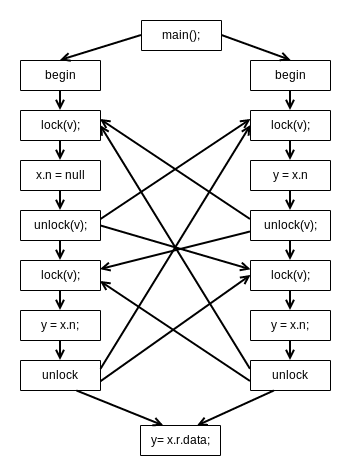
\includegraphics[width=0.5\textwidth]{Figures/hra_live_concurrent.png}
	\caption{Concurrent Heap liveness analysis input}
	\label{fig:nullpointeranalysis}
\end{figure}     

